\documentclass[article]{IEEEtran}
\IEEEoverridecommandlockouts
% The preceding line is only needed to identify funding in the first footnote. If that is unneeded, please comment it out.
\usepackage{cite}
\usepackage{amsmath,amssymb,amsfonts}
\usepackage{algorithmic}
\usepackage{graphicx}
\usepackage{textcomp}
\usepackage{xcolor}

\usepackage[utf8]{inputenc}
\usepackage[T1]{fontenc}
\usepackage[spanish]{babel}
\usepackage{hyperref}
\usepackage{booktabs}
\graphicspath{ {imagenes/} }
\hypersetup{
    colorlinks=true,
    linkcolor=blue,
    filecolor=magenta,      
    urlcolor=cyan
}


\def\BibTeX{{\rm B\kern-.05em{\sc i\kern-.025em b}\kern-.08em
    T\kern-.1667em\lower.7ex\hbox{E}\kern-.125emX}}
\begin{document}

\title{Modelado y Simulación de \emph{Middleware} Orientado a Mensajes: Un enfoque exploratorio basado en componentes \\
%{\footnotesize \textsuperscript{*}Note: Sub-titles are not captured in Xplore and
%should not be used}
%\thanks{Identify applicable funding agency here. If none, delete this.}
}

\author{\IEEEauthorblockN{Carlos Martín Flores González}
\IEEEauthorblockA{\textit{Escuela de Ingeniería en Computación} \\
\textit{Tecnológico de Costa Rica}\\
Cartago, Costa Rica \\
\texttt{mfloresg@ieee.org}}
}

\maketitle

\begin{abstract}
This document is a model and instructions for \LaTeX.
This and the IEEEtran.cls file define the components of your paper [title, text, heads, etc.]. *CRITICAL: Do Not Use Symbols, Special Characters, Footnotes, 
or Math in Paper Title or Abstract.
\end{abstract}

\renewcommand\IEEEkeywordsname{Palabras Clave}
\begin{IEEEkeywords}
component, formatting, style, styling, insert
\end{IEEEkeywords}

\section{Introducción}
\IEEEPARstart{L}{os} métodos de predicción de rendimiento basados en modelos permiten a los arquitectos de software evaluar el rendimiento de los sistemas de software durante las primeras etapas de desarrollo. Estos modelos de predicción se centran en los aspectos relevantes de la arquitectura y de la lógica del negocio, dejando de lado detalles de la infraestructura subyacente. Sin embargo, estos detalles son esenciales para generar predicciones de rendimiento que sean precisas.

Para los ingenieros, es una práctica común simular el modelo de un artefacto antes de construirlo. Modelos de diseños de autos, circuitos electrónicos, puentes, entre otros, son simulados para entender el impacto de decisiones de diseño en varias atributos de calidad de interés como seguridad, consumo de energía o estabilidad. La habilidad de predecir las propiedades de un artefacto en base a su diseño sin necesidad de construirlo, es una de las características centrales de una disciplina de ingeniería. A partir de esta visión de lo que se considera una disciplina de ingeniería establecida se podría decir entonces que la ingeniería de software es apenas una disciplina de ingeniería\cite{palladio-blue-book}. Esto porque frecuentemente los ingenieros de software carecen del entendimiento del impacto de decisiones de diseño en atributos de calidad como rendimiento o confiabilidad. Como resultado, se intenta probar la calidad del software mediante costosos ciclos de prueba y error.

El no entender el impacto en las decisiones de diseño puede ser costoso y riesgoso. Probar software significa que ya se ha hecho un esfuerzo en su implementación. Por ejemplo, si las pruebas revelan problemas de rendimiento, es muy probable que la arquitectura necesita ser modificada, lo que puede conllevar a costos adicionales. Estos costos surgen debido a que en sistemas de software empresarial un bajo rendimiento es principalmente el efecto de una arquitectura inadecuada que efecto de código.

La ingeniería de rendimiento de software(SPE por sus siglas en inglés) es una disciplina que se centra en incorporar aspecto de rendimiento dentro del proceso de desarrollo de software, con el objetivo de entregar software de confiable de acuerdo con propiedades de rendimiento particulares. Los modelos de rendimiento predictivos son una de las herramientas empleadas en SPE. Construidos en las fases tempranas del proceso de desarrollo de software, los modelos ayudan a predecir el rendimiento eventual del software y de esta forma guiar el desarrollo, para eso los modelos de predicción de rendimiento deben capturar todos los componentes relevantes del sistema.

Para aplicaciones de software moderans, esto puede implicar modelar complejas capas tales como máquinas virtuales o \emph{middleware} de mensajería. Componer todos estos modelos puede resultar una tarea costosa e ineficiente. En su lugar, un modelo abstracto de la aplicación se puede construir primero y luego ir agregando los modelos de los componentes del sistema. 

En este trabajo se propone la construcción de un modelo de rendimiento para un sistema que utilice \emph{middleware} orientado a mensajes con el fin de evaluar la influencia en el rendimiento de dicho sistema. Se propone evaluar esta influencia por medio de un ejemplo: tomar una aplicación de referencia con el fin de obtener sus métricas actuales de rendimiento, adaptarla para que utilice \emph{middleware} orientado a mensajes y luego medir su rendimiento y generar un modelo a partir de esto.  

Este artículo está organizado de la siguiente manera: la Sección \ref{sec:trabajos-relacionados} presenta trabajos relacionados al estudio del rendimiento de MOM utilizando modelado y simulación. La Sección \ref{sec:spe} introduce a la ingeniería de rendimiento de software, características y al \emph{Palladio Component Model} (PCM). La Sección \ref{sec:mom} se dedica al \emph{Middleware} orientado a mensajes. \emph{CloudStore}, la aplicación que se tomará como referencia para evaluar la influencia de MOM se presenta en la Sección \ref{sec:cloudstore}. Los resultados de la modificación del modelo PCM y la aplicación se dan a conocer en la Sección \ref{sec:resultados}. En artículo concluye en la Sección \ref{sec:conclusion}.

\section{Trabajos Relacionados} \label{sec:trabajos-relacionados}
En \cite{happe-et-al} se extiende el \emph{Palladio Component Model} con \emph{performance completions} para \emph{middleware} orientado a mensajes. \emph{Performance completions}\cite{woodside-et-al-2} proporcionan el concepto general de incluir detalles de bajo nivel de ambientes de ejecución en modelos de rendimiento. Con la extensión del modelo, los arquitectos de software puede especificar y configurar comunicación basada en mensajes utilizando un lenguaje basado en patrones de mensajería.

La influencia en el rendimiento de \emph{middleware} orientado a mensajes fue estudiada en \cite{liu-gordon}. Se consideró el \emph{middleware} como un factor determinante del rendimiento en sistemas distribuidos y se hizo un mayor enfoque en su modelado y evaluación. Se propuso un enfoque basado en medición en combinación con modelos matemáticos para predecir el rendimiento de aplicaciones J2EE\footnote{\emph{Java Enterprise Edition}}. Las mediciones proporcionan los datos necesarios para calcular los valores de entrada de un modelo de red de cola(\emph{queueing network model}). El cálculo refleja el comportamiento de la aplicación en cuestión. La red de cola se resuelve para derivar métricas de rendimiento tales como tiempos de respuesta y \emph{throughput} de la aplicación. 

La investigación llevada a cabo en \cite{chew} presenta un modelo abstracto de \emph{middleware} orientado a mensajes basado en Apache Qpid junto con el uso de modelos exógenos de autorregressión (ARX por sus siglas en inglés) que describen el comportamiento del \emph{middleware} durante condiciones de cuellos de botella. Los modelos ARX son modelos autorregresivos en donde la salida depende de la salida anterior así como de estimulos externos. Estos componentes son integrados para producir una técnica generalizada de calibración para rendimiento del \emph{middleware} y detección de cuellos de botella en el mismo.

En \cite{martinec-et-al} se construyen modelos de rendimiento para \emph{middleware} que implementa el estándar JMS\footnote{\emph{Java Messaging Service}}. Se utiliza análisis de código y mediciones experimentales de implementaciones de JMS populares para mostrar situaciones en las que el rendimiento observado no es predecido de forma precisa por otros modelos. Se proporciona un análisis técnico detallado de los efectos observados como base para futuros trabajos de modelado. Por último, se diseña un modelo de rendimiento que captura estos efectos y se valida el modelo utilizando mediciones experimentales.

Un modelo analítico $M/M/1$ con políticas \emph{first in - first out} y prioridad de colas fue diseñado y desarrolloado en \cite{alwakeel} para evaluar el rendimiento de \emph{middleware} orientado a mensajes y llamados a procedimientos remotos (RPC por sus siglas en inglés). Los modelos comparan el rendimiento de \emph{middleware} orientado a mensajes y RPC con prioridad de colas y analizan el \emph{throughput} de estos paradigmas de comunicación. Varios parámetros de entrada son usados para determinar la configuración óptima para lograr el máximo rendimiento. Los resultados prueban que al utilizar \emph{middleware} orientado a mensajes con prioridad de cola, el \emph{throughput} del sistema puede ser mejorado. 

\section{Ingeniería de Rendimiento de Software (\emph{Software Performance Engineering -- SPE})} \label{sec:spe}
Una definición comúnmente utilizada para definir ingeniería de rendimiento de software es la que que brinda Woodside \cite{woodside-et-al}: \emph{``Ingeniería de rendimiento de software representa toda la colección de actividades de ingeniería de sofware y análisis relacionados utilizadas a través del ciclo de desarrollo de software, que están dirigidos a cumplir con los requisitos de rendimiento''}. 

De acuerdo con este mismo autor, los enfoques para ingeniería de rendimiento puede ser divididos en dos categorías: basadas en mediciones y basadas en modelos. La primera es la más común y utiliza pruebas, diagnóstico y ajustes una vez que existe un sistema en ejecución que se puede medir, es por esto que solamente puede ser utilizada conforme se va acercando el final del ciclo de desarrollo de software. Al contrario del enfoque basado en mediciones, el enfoque basado en modelos se centra en las etapas iniciales del desarrollo. Como el nombre lo indica, en este enfoque los modelos son clave para hacer predicciones cuantitativas de qué tan bien una arquitectura puede cumplir sus expectativas de rendimiento.

Se han propuesto otras clasificaciones de enfoques para SPE pero, con respecto a la evaluación de sistemas basados en componentes, en \cite{performance-model-survey} se deja la clasificación a un lado debido a que se argumenta que la mayoría de enfoques de modelaje toman alguna medición como entrada y a la mayoría de los métodos de medición los acompaña algún modelo.

\subsubsection{Ingeniería de rendimiento basada en mediciones}
Los enfoques basados en mediciones prevalencen en la industria\cite{thijmen-thesis} y son típicamente utilizados para verificación(¿el sistema cumple con su requisito de rendimiento?) o para localizar y arreglar \emph{hot-spots} (cuáles son las partes que tienen peor rendimiento en el sistema). La medición de rendimiento se remonta al inicio de la era de la computación, lo que ha generado una amplia gama de herramientas como generadores de carga y monitores para crear cargas de trabajo ficticias y llevar a cabo la medición de un sistema respectivamente.

Las pruebas de rendimiento aplican técnicas basadas en medición y usualmente esto es hecho luego de las pruebas funcionales o de carga. Las pruebas de carga verifican el funcionamiento de un sistema bajo cargas de trabajo pesadas, mientras que las pruebas de rendimiento son usadas para obtener datos cuantitativos de características de rendimiento, como tiempos de respuesta, \emph{throughput} y utilización de hardware para una configuración de un sistema bajo una carga de trabajo definida.

\subsection{Ingeniería de rendimiento a través de modelado} 
La importancia del modelado del rendimiento está motivada por el riesgo de problemas graves de rendimiento\cite{palladion-screencast} y la creciente complejidad de sistemas modernos, lo que hace difícil abordar los problemas de rendimiento al nivel de código. Cambios considerables en el diseño o en las arquitecturas pueden ser requeridos para mitigar los problemas de rendimiento. Por esta razón, la comunidad de investigación de modelado de rendimiento intenta luchar contra el enfoque de ``arreglar las cosas luego'' durante el proceso de desarrollo. Con la aplicación de modelo del rendimiento de software se busca encontrar problemas de rendimiento y alternativas de diseño de manera temprana en el ciclo de desarrollo, evitando así el costo y la complejidad de un rediseño o cambios en los requerimientos.

Las herramientas de modelado de rendimiento ayudar a predecir la conducta del sistema antes que este sea construido o bien, evaluar el resultado de un cambio antes de su implementación. El modelado del rendimiento puede ser usado como una herramienta de alerta temprana durante todo el ciclo de desarrollo con mayor precisión y modelos cada vez más detallados a lo largo del proceso. Al inicio del desarrollo un modelo no puede ser validado contra un sistema real, por esto el modelo representa el conocimiento incierto del diseñador. Como consecuencia de esto el modelo hace suposiciones que no necesariamente se van a dar en el sistema real, pero que van a ser útiles para obtener una abstracción del comportamiento del sistema. En estas fases iniciales, la validación se obtiene mediante el uso del modelo, y existe el riesgo de conclusiones erróneas debido a su precisión limitada. Luego, el modelo puede ser validado contra mediciones en el sistema real (o parte de este) o prototipos y esto hace que la precisión del modelo se incremente.

En \cite{jit-et-al} se sugiere que los métodos actuales tienen que superar un número de retos antes que puedan ser aplicados en sistemas existentes que enfrentan cambios en su arquitectura o requerimientos. Primero, debe quedar claro cómo se obtienen los valores para los parámetros del modelo y cómo se pueden validar los supuestos. Estimaciones basadas en la experiencia para estos parámetros no son suficientes y mediciones en el sistema existente son necesarias para hacer predicciones precisas. Segundo, la caracterización de la carga del sistema en un entorno de producción es problemática debido a los recursos compartidos (bases de datos, hardware). Tercero, deben desarrollarse métodos para capturar parámetros del modelo dependientes de la carga. Por ejemplo un incremento en el tamaño de la base de datos probablemente incrementará las necesidades de procesador, memoria y disco en el servidor.

Técnicas comúnes de modelado incluyen redes de colas, extensiones de estas como redes de colas en capas y varios tipos de redes de Petri y procesos de álgebra estocástica.


\subsection{Modelado de Rendimiento}
En SPE, la creación y evaluación de modelos de rendimiento es un concepto clave para evaluar cuantitativamente el rendimiento del diseño de un sistema y predecir el rendimiento de otras alternativas de diseño. Un modelo de rendimiento captura el comportamiento relevante al rendimiento de un sistema para identificar el efecto de cambios en la configuración o en la carga de trabajo en el rendimiento. Permite predecir los efectos de tales cambios sin necesidad de implementación y ejecución en un ambiente de producción, que podrían ser no solamente tareas costosas sino también un desperdicio en el caso que un el hardware con el que se cuenta pruebe ser insuficiente para soportar la intensidad de la carga de trabajo.\cite{noorshams}

La forma del modelo de rendimiento puede comprender desde funciones matemáticas a formalismos de modelado estructural y modelos de simulación. Estos modelos varían en sus características clave, por ejemplo, las suposiciones de modelado de los formalismos, el esfuerzo de modelado requerido y el nivel de abstracción.

En cuanto a técnicas de simulación, a pesar que estas permiten un estudio más detallado de los sistemas que modelos analíticos, la construcción de un modelo de simulación requiere de conocimiento detallado tanto de desarrollo de software como de estadística\cite{thijmen-thesis}. Los modelos de simulación también requieren usualmente de mayor tiempo de desarrollo que los modelos analíticos. En \cite{woodside-et-al} se menciona que ``la construcción de un modelo de simulación es caro, algunas veces comparable con el desarrollo de un sistema, y, los modelos de simulación detallados puede tardar casi tanto en ejecutarse como el sistema.

\subsection{Modelado de Arquitecturas de Software con Palladio Component Model}
El \emph{Palladio Component Model (PCM)} es un enfoque de modelaje para arquitecturas de software basados en componentes que permite predicción de rendimiento basada en modelos. PCM contribuye al proceso de desarrollo de ingeniería basado en componentes y proporciona conceptos de modelaje para describir componentes de software, arquitectura de software, despliegue (\emph{deployment}) de componentes y perfiles de uso de sistemas de software basados en componentes en diferentes submodelos (Figura \ref{fig:pcm-instance}).

\begin{figure*}[h]
  \centering
  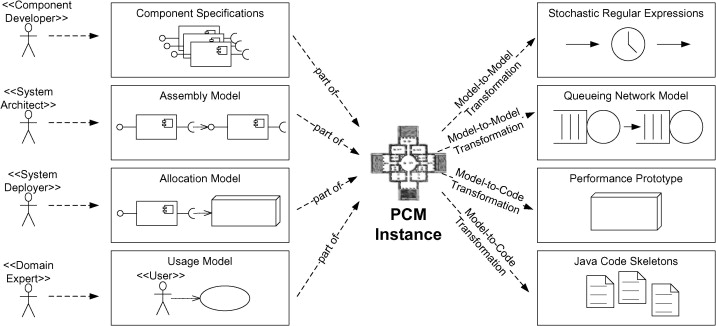
\includegraphics[width=12cm]{palladio-cbse-process}
  \caption{\small{Instancia de un modelo PCM. Tomado de \cite{happe-et-al}}}
  \label{fig:pcm-instance}
\end{figure*} 

\begin{itemize}
    \item \textbf{Especificaciones de componentes} son descripciones abstractas y paramétricas de los componentes de software. En las especificaciones de software se proporciona una descripción del comportamiento interno del componente así como las demandas de sus recursos en RDSEFFs (\emph{Resource Demanding Service EFFect specifications}) utilizando una sintaxis similar a los diagramas de actividad de UML.
    \item \textbf{Un modelo de ensamblaje} (\emph{assembly model}) especifica qué tipo de componentes se utilizan en una instancia de aplicación modelada y si las instancias del componente se replican. Además, define cómo las instancias del componente se conectan representando la arquitectura de software.
    \item El entorno de ejecución y los recursos, así como el despliegue (\emph{deployment}) de instancias de componentes para dichos contenedores de recursos se definen en un \textbf{modelo de asignación} (\emph{allocation model}).
    \item El \textbf{modelo del uso} especifica la interacción de los usuarios con el sistema utilizando una sintaxis similar al diagrama de actividades de UML proporcionando una descripción abstracta de la secuencia y la frencuencia en que los usuarios activan las operaciones disponibles en un sistema.
\end{itemize}

Un modelo PCM abstrae un sistema de software a nivel de arquitectura y se anota con consumos de recursos que fueron medidos previamente u otros que son estimados. El modelo puede entonces ser usado en transformaciones de modelo-a-modelo o modelo-a-texto a un modelo de análisis en particular (redes de colas o simulación de código) que puede ser analíticamente resuelto o simulado para obtener resultados sobre el rendimiento y predicciones del sistema modelado. Los resultados del rendimiento y las predicciones pueden ser utilizadas como retroalimentación para evaluar y mejorar el diseño inicial, permitiendo así una evaluación de calidad de los sistemas de software en base a un modelo\cite{noorshams}. 

\section{\emph{Middleware} Orientado a Mensajes} \label{sec:mom}
Junto con el crecimiento de Internet, los sistemas distribuidos han crecido a una escala masiva. Hoy en día, estos sistemas puede involucrar a miles de entidades distruidas globalmente. Esto ha motivado el estudio de modelos de comunicación y sistemas flexibles, que puedan reflejar la naturaleza dinámica y desacoplada de las aplicaciones.

La integración de tecnologías heterogéneas es una de las áreas principales en donde la comunicación basada en mensajes juega un papel clave. Más y más compañías se enfrentan al problema de integrar sistemas y aplicaciones heterogéneas dentro y fuera de la organización ya sea por fusiones, adquisiciones, requisitos comerciales o simplemente un cambio en la direción tecnológica. No es raro encontrar una gran cantidad de tecnologías y plataformas dentro de una solo compañía, desde productos de código libre y comerciales hasta sistemas y equipos heredados (\emph{legacy}).

La comunicación basada en mensajes también ofrece la habilidad de procesar solicitudes de manera asincrónica, proporcionando a los arquitectos y desarrolladores soluciones para reducir o eliminar cuellos de botella en un sistema e incrementar la productividad del usuario final y del sistema en general. Dado que la comunicación basada en mensajes provee un alto grado de desacoplamiento entre componentes, los sistemas que utilizan esta tecnología también logran contar con altos grados de agilidad y flexibilidad en su arquitectura.

A los sistemas de mensajería de aplicación-a-aplicación que se utilizan sistemas de negocios se les denomina genéricamente sistemas de mensajería empresarial o \emph{middleware} orientado a mensajes\cite{jms20}. MOM permite a dos o más aplicaciones intercambiar información en forma de mensajes. Un mensaje en este caso es un paquete autocontenido de datos de negocio y encabezados de enrutamiento de red. Los datos de negocio contenidos en un mensaje puede ser cualquier cosa, van a depender de cada negocio, y usualmente contiene información acerca de algún tipo de transacción. En sistemas de mensajería empresariales, los mensajes informan a una aplicación de la ocurrencia de algún evento en otro sistema. La tasa de mensajes depende de la capacidad de la implementación de MOM o \emph{broker}. El retraso depende de la latencia en el \emph{broker} y en los caminos de entrada y salida\cite{chew}.

Al usar MOM, los mensajes son trasmitidos desde una aplicación a otra a través de la red. Productos de \emph{middleware} empresarial aseguran que los mensajes se distribuyan correctamente entre las aplicaciones. Además estos productos usualmente proporcionan tolerancia a fallos, balanceo de carga, escalabilidad y soporte transaccional para sistemas que necesitan que necesitan intercambiar de manera confiable grandes cantidades de mensajes.

Los fabricantes de MOM usan diferentes formatos de mensajes y protocolos de red para intercambiar mensajes pero la semántica básica es la misma. Una interfaz de programación (un API, por sus siglas en inglés) se utiliza para crear un mensaje, cargar los datos, asignar información de enrutamiento y enviar el mensaje. La misma API se utiliza para recibir los mensajes producidos por otras aplicaciones.

En todos los sistemas modernos de mensajería empresarial, las aplicaciones intercambian mensajes a través de canales virtuales llamados destinos(\emph{destinations}). Cuando un mensaje se envía, se dirije a un destino (por ejemplo una cola o un tópico) no a una aplicación específica. Cualquier aplicación que subscriba o registre un interés en ese destino puede recibir el mensaje. De esta forma, las aplicaciones que reciben mensajes y aquellas que envían mensajes están desacopladas. Los emisores y receptores no están enlazados uno con otro de ninguna forma y pueden enviar y recibir mensajes como mejor les parezca.

Un concepto clave de MOM es que los mensajes son entregados de forma asincrónica desde un sistema a otros sobre la red. El entregar un mensaje de manera asicrónica significa que el emisor no requiere esperar a que el mensaje sea recibido o manejado por el receptor, él es libre de enviar el mensaje y continuar su procesamiento. Los mensajes asicrónicos son tratados como unidades autónomas: cada mensaje es autocontenido y lleva consigo todos los datos necesarios para ser procesado.

En comunicación de mensajes asincrónicos, las aplicaciones usan una API para construir un mensaje, luego pasarlos al MOM para su entrega a uno o varios recipientes (Figura \ref{fig:mom}). Un mensaje es un paquete de datos que es enviado desde una aplicación a otra sobre la red. El mensaje debe de ser autodescriptivo en el sentido que debe de contener todo el contexto necesario para que permit a los recipientes llevar a cabo su trabajo de forma independiente. 

\begin{figure}[h]
  \centering
  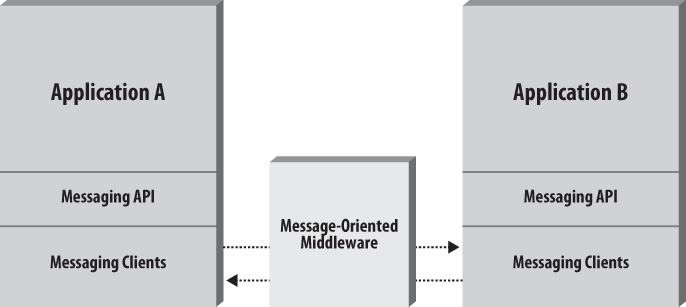
\includegraphics[width=9cm]{jms20-mom}
  \caption{\small{\emph{Middleware} Orientado a Mensajes. Tomado de \cite{jms20}}}
  \label{fig:mom}
\end{figure}

La arquitecturas de MOM de hoy en día varían en su implementación. Van desde las arquitecturas centralizadas que dependen de un servidor de mensajes para realizar enrutamiento a arquitecturas descentralizadas que distribuyen el procesamiento del servidor hacia los clientes. Una variedad de protocolos como \texttt{TCP/IP, HTTP, SSL} y \texttt{IP} son empleados como capa de transporte de red.

Los sistemas de mensajería están compuestos por clientes de mensajería (\emph{messaging clients}) y algún tipo de servidor MOM. Los clientes envían mensajes al servidor de mensajería el cual distribuye estos mensajes a otros clientes. El cliente es una aplicación de negocio o componente que es usa una API de mensajería.

\subsubsection{Punto-a-Punto}
Este modelo de mensajería permite a los clientes enviar y recibir mensajes de forma síncrona como asíncrona a través de canales virtuales conocidos como colas. En este modelo a los productores de mensajes se les llama emisores (\emph{senders}) y a los consumidores se les conoce como receptores (\emph{receivers}). El modelo punto-a-punto ha sido tradicionalmente un modelo basado en \emph{polling}, en donde los mensajes son solicitados desde la cola en lugar de ser puestos en el cliente automáticamente. Los mensajes que se envían a una cola son recibidos por uno y solo un \emph{receiver}, aunque pueden haber otros \emph{receivers} escuchando en la cola por el mismo mensaje. Este es un modelo que promueve acoplamiento esto porque generalmente el \emph{sender} conocer cómo el mensaje va a ser utilizado y quién lo va a recibir. 

\subsubsection{Publish-and-Subscribe}
En este modelo, los mensajes son publicados en un canal virtual llamado tópico. Los productores de mensajes son conocidos como \emph{publishers} y a los consumidores se les llama \emph{subscribers}. Los mensajes pueden ser recibidios por múltiples \emph{subscribers}, a diferencia del modelo punto-a-punto. Cada \emph{subscriber} recibe una copia de cada mensaje. Este es un modelo basado en \emph{push} en donde los mensajes son automáticamente transmitidos a los consumidores sin que estos tengan que solicitarlos o revisar la cola por nuevos mensajes. 

Este modelo tiende a ser menos acoplado que el modelo punto-a-punto debido a que el publicador del mensaje generalmente no está conciente de cuántos subscritores hay y lo qué van a hacer estos con el mensaje. 

\section{Modelado de rendimiento en una Aplicación: \emph{CloudStore}} \label{sec:cloudstore}

\subsection{CloudStore} 
Con el fin de explorar la aplicabilidad de modelaje basado en componentes en aplicaciones que utilizan MOM, se inició la búsqueda de una aplicación de referencia existente que haya sido modelada a partir de PCM. De esta forma, se contaría con una base la cual se podría modificar y evaluar cuando se le introduzca un MOM. Para seleccionar una aplicación que se adecue al tema propuesto, se establecieron los siguientes criterios:
\begin{enumerate}
    \item Aplicación de código libre
    \item Que cuente con modelos de rendimiento hechos en \emph{Palladio Component Model}
    \item Desarrollada en un lenguaje de programación y con herramientas de actualidad
    \item Que continue siendo mantenida y mejorada por sus autores
\end{enumerate}
Del listado anterior, quizás el criterio más restrictivo es el \#2 pero al mismo tiempo se considera el de mayor importancia debido a que en esta investigación se están dando los primeros pasos con el modelado de arquitecturas utilizando Palladio y no se deseaba empezar desde cero sino más bien tomar un modelo de referencia e ir haciendo pequeñas modificaciones y probar los resultados.

\emph{CloudScale}\cite{cloudscale-2}, un proyecto generado a partir de la experiencia de Palladio, es un método que permite identificar y gradualmente resolver problemas de escalabilidad en aplicaciones existentes. \emph{CloudScale} también permite modelar alternativas de diseño y el análisis de su efecto en la escalibilidad y costo\cite{cloudscale}. El sitio Web de \emph{CloudScale}, \url{http://www.cloudscale-project.eu/} contiene publicaciones e información general acerca de este método, así también como del \emph{CloudScale Environment}, un entorno de desarrollo integrado creado para modelaje y análisis. 

Con el fin de validar \emph{CloudScale}, varias aplicaciones fueron creadas. Una ventaja de las aplicaciones que utlizan \emph{CloudScale} es que deben de tener un modelos de componentes, de su utilización, de los recursos, el sistema y uso basados en PCM para su posterior procesamiento. Otra de las cosas que hicieron que las aplicaciones creadas para esta metología resultaran atractivas para esta investigación, es que el proyecto \emph{CloudScale} es reciente por lo que estas aplicaciones no se consideran como ``viejas'' y se les da mantenimiento.

Una de estas aplicaciones que se crearon para probar esta metolodología es \emph{CloudStore}, una aplicación Web de código libre que emula una tienda (\emph{e-commerce}) de libros en línea. Su objetivo principal es ser utilizada para el análisis de las características de los sistemas en la nube como escalabilidad, capacidad, elasticidad y eficiencia. Fue desarrollada como la aplicación de muestra para validar las herramientas de \emph{CloudScale}. 

La aplicación fue desarrollada en Java utilizando la librerías de \emph{Spring} y se ejecuta en un servidor Tomcat. Utiliza una base de datos MySQL. Para mayor información sobre \emph{CloudStore}, se puede visitar su repositorio en GitHub: \url{https://github.com/CloudScale-Project/CloudStore}.

\begin{figure}[h]
  \centering
  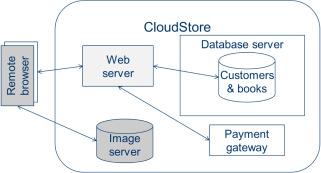
\includegraphics[width=9cm]{conceptual-cloudstore-architecture}
  \caption{\small{Arquitectura Conceptual de CloudStore. Tomado de \cite{cloudscale-2}}}
  \label{fig:cloudstore-conceptual}
\end{figure}

En la figura \ref{fig:cloudstore-conceptual} se muestra la arquitectura conceptual de \emph{CloudStore}. Tiene un diseño simple: una aplicación Java que se ejecuta en un servidor Web y que realiza consultas a una base de datos MySQL. Para llevar a cabo los pagos, la aplicación se comunica con un \emph{gateway} para pagos, un servicio Web publicado en un servidor externo al del \emph{CloudStore} que simula el tiempo de respuesta de podría tomar realizar un pago.

Una característica de \emph{CloudStore} particularmente atractiva para este estudio es precisamente el \emph{gateway} de pagos. La interacción entre \emph{CloudStore} y este \emph{gateway} de pagos representa un clásico escenario de integración de sistemas. En su versión original, \emph{CloudStore} realiza llamadas a este \emph{gateway} de pagos de manera \emph{ad hoc} y es aquí en donde la introducción de comunicación basada en mensajes puede ser una mejor opción al actual debido que:
\begin{itemize}
    \item Permite que \emph{CloudStore} se desacople del \emph{gateway} de pagos: la aplicación no necesita saber información específica de este \emph{gateway} ni la forma en cómo debe interactuar con él, esto se lo delega a un tercero. 
    \item La comunicación basada en mensajes puede garantizar el envío de peticiones al gateway de pagos.
\end{itemize}

\subsection{Adaptación de \emph{CloudStore}}
Con el fin de adaptar \emph{CloudStore} para que soporte comunicación basada en mensajes cuando se ejecute un pago, se propone lo siguiente:
\begin{enumerate}
    \item Selección de una solución para comunicación basada en mensajes
    \item Selección de librería(s) de código para realizar comunicación entre \emph{CloudStore} y la solución seleccionada en el punto anterior
    \item Implementar un consumidor de mensajes de petición de pago: una aplicación que estará monitoreando(\emph{pooling}) y procesando mensajes provenientes de la solución seleccionada en el punto \#1 y que los entregará al \emph{gateway} de pagos. Adicionalmente esta aplicación comunicará al \emph{CloudStore} el estado del procesamiento del pago
    \item Reemplazar el código existente que se dedica a realizar el pago contra el \emph{gateway} de pagos por nuevo código que se comunicará con la solución de mensajería
\end{enumerate}

Para el punto \#1, se seleccionó ActiveMQ\footnote{\url{http://activemq.apache.org/}}, el servidor más popular de mensajería de código libre.
 
Al estar utlizando ActiveMQ, el cual es un servidor que implementa el estándar \emph{Java Messaging Service}, se va a utilizar la librería \texttt{javax.jms} con versión 1.1.

La aplicación consumidora/procesadora de mensajes será una aplicación Java que se va a ejecutar como un servicio. 

\begin{figure*}[h]
  \centering
  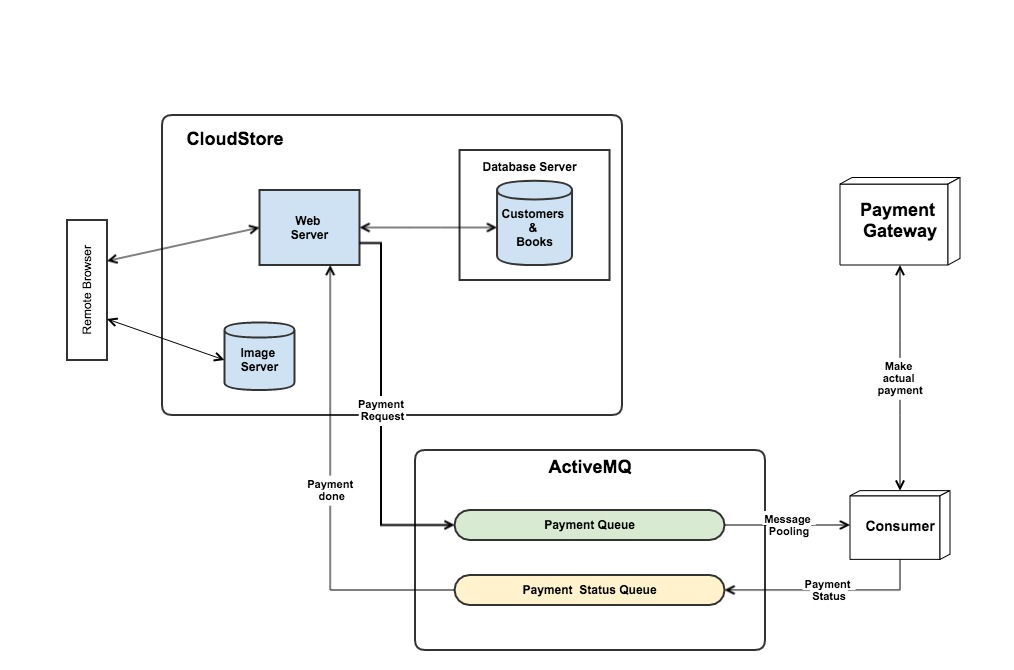
\includegraphics[width=14cm]{cloudstore-jms}
  \caption{\small{Arquitectura Conceptual de CloudStore utilizando comunicación basada en mensajería}}
  \label{fig:cloudstore-jms}
\end{figure*}

La arquitectura adaptada de \emph{CloudStore} para que utilice comunicación basada en mensajes se muestra en la figura \ref{fig:cloudstore-jms}. Ahora, en lugar de realizar una llamada \emph{ad hoc} al \emph{gateway} de pagos, la aplicación se comunica con una cola de mensajería para pagos tanto para el envío como para la recepción del pago. A este esquema de comunicación se le conoce como \emph{request-reply}, esto porque la aplicación que inicia la petición se queda a la espera del resultado.

Para realizar un pago, \emph{CloudStore} enviará un mensaje a una cola de pagos, en la figura \ref{fig:cloudstore-jms} se identifica como ``Payment Queue''. La aplicación consumidora de mensajes, estará monitoreando esta cola constantemente con el fin de tomar los mensajes y procesarlos contra el \emph{gateway} de pagos. Una vez que el pago se haya efectuado, la aplicación consumidora envía el resultado del pago a otra cola identificada en la figura \ref{fig:cloudstore-jms} como ``Payment Status Queue''. \emph{CloudStore} estará monitoreando los mensajes provenientes de esta cola con el fin de conocer el estado del pago.

\subsubsection{Aplicación original \emph{vs.} Aplicación modificada}
Se siguieron las instrucciones proporcionadas en los repositorios de código para la puesta en ejecución de \emph{CloudStore}: instalación dependencias de código necesarias y creación de \emph{scripts} para crear la base de datos y agregar registros a la misma. Una vez que la aplicación se construyó y se configuró para que trabajara junto con una base de datos MySQL local, la misma se pudo ejecutar en el puerto \texttt{:8080}.

Luego de ejecutar la aplicación localmente y probar que funcione adecuadamente, se procedió a crear un ambiente de producción en Amazon AWS. Para esto, se creó un ambiente con un servidor Apache Tomcat 8 y una base de datos MySQL utilizando los servicios de \emph{Elastic BeanStalk} y \emph{Relational Database Services}(RDS) respectivamente. A este ambiente se llamó \texttt{cloudstore-plain}. Se configuró la aplicación para que cuando fuera instalada en este ambiente se conectara a la base de datos en AWS.

Cuando ambas, la aplicación local y la instalada en AWS pudieron ser ejecutarse satisfactoriamente, se empezó con la adaptación de \emph{CloudStore}. Lo primero fue instalar e iniciar una instancia de ActiveMQ localmente. En su configuración por defecto, ActiveMQ se ejecuta en el puerto \texttt{:61616} y su aplicación Web de administración en el puerto \texttt{:8161}. Se crearon dos colas de mensajes: \texttt{payment-queue}, en donde se enviarán los mensajes(peticiones) de pago y \texttt{payment-status-queue}, en donde se enviarán los mensajes del estado del pago.  Luego se hizo un nuevo \emph{branch} (rama) en el repositorio de código para los nuevos cambios que se iban a realizar. Este \emph{branch} lleva por nombre \texttt{jms}. Se instaló la dependencia \texttt{javax.jms 1.1} para que la aplicación pudiera comunicarse por medio del estándar \emph{Java Messaging Service}. Se cambió el flujo de trabajo de \emph{CloudStore} para que en lugar de llamar al \emph{gateway} de pago de manera \emph{ad hoc}, se creará un mensaje con la información de la compra para luego enviar este a la cola de mensajes \texttt{payment-queue}. Por último, se agregará código para monitorear y consumir el resultado del pago, el cual debería de ser entregado por la cola \texttt{payment-status-queue}. A este estilo de comunicación se le conoce como \emph{request-reply}: la parte que envia la comunicación debe de aportar algún tipo de encabezado y/o meta-dato al mensaje para su posterior identificación. Luego de enviar el mensaje, la aplicación se pone en modo de monitoreo para filtrar y procesar solamente aquellos mensajes que fueron generados por esta.

Se creó un nuevo proyecto en Java llamado \texttt{jms-receiver}. Este nuevo proyecto va a llevar a cabo las siguientes actividades: monitoreo y consumo constante de mensajes de la cola \texttt{payment-queue}, realizar una llamada al \emph{gateway} de pagos, obtener el resultado del pago y enviarlo por la cola \texttt{payment-status-queue}.

Primero se probaron los cambios localmente y se pudo comprobar como ahora los mensajes con las peticiones de pagos viajaban a través de las colas de mensajería en lugar de ser generadas a lo interno de \emph{CloudStore}.

Para poner estos nuevos cambios en un ambiente de producción se realizaron las siguientes actividades:
\begin{itemize}
    \item Se creó un nuevo ambiente en \emph{Elastic BeanStalk} llamado \texttt{cloudstore-jms}
    \begin{itemize}
        \item En este nuevo ambiente se va a instalar la aplicación de \emph{CloudStore} modificada que vive en el \emph{branch} \texttt{jms}.
    \end{itemize}

    \item Se provisionó una nueva máquina virtual en el servicio \emph{Amazon Elastic Compute Cloud} (EC2). Una máquina virtual con Ubuntu 16.04, Java y ActiveMQ
    \begin{itemize}
        \item En esta máquina virtual se va a ejecutar la aplicación \texttt{jms-receiver} y el servicio de ActiveMQ con las colas de \texttt{payment-service} y \texttt{paymente-status-queue}
    \end{itemize}
    \item Se configuró la versión de \emph{CloudStore} modificada para que se comunicara con las colas de mensajería que se encuentran en la nueva máquina virtual provisionada
\end{itemize}

A continuación se presentan las dos versiones de \emph{CloudStore} ejecutándose en un ambiente de producción. En la figura \ref{fig:aws-cs-plain} se muestra la versión original de \emph{CloudStore} ejecutándose en un ambiente de producción. La aplicación modificada luce similar a la original, pero apuntan a dominios diferentes y también difieren en la forma en la que se realiza el proceso de pago

\begin{figure}[h]
  \centering
  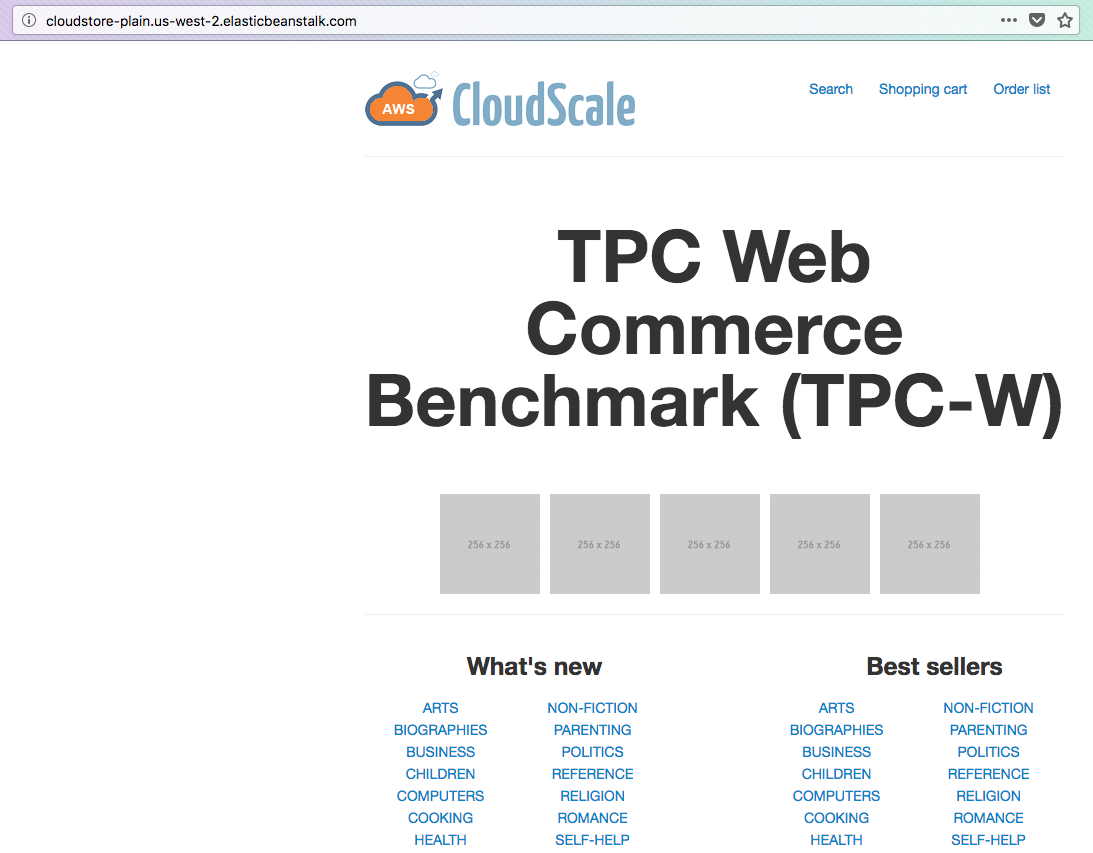
\includegraphics[width=9cm]{aws-cs-plain}
  \caption{\small{Versión original de \emph{CloudStore} (\emph{cloudstore-plain}) en AWS}}
  \label{fig:aws-cs-plain}
\end{figure}

\subsection{Modelado de MOM en CloudStore} \label{sec:cloudstore-mom}
El modelo PCM de \emph{CloudStore} se tiene que modificar para reflejar que hay un nuevo(s) componente(s) para soportar comunicación basada en mensajes. Se reemplaza el componente \emph{PaymentGateway} del modelo original por nuevos componentes para envío y recepción de mensajes propuestos en \cite{happe-et-al}. En \cite{happe-et-al}, se propone la creación de una ``plantilla'' para generar modelos de MOMs. Para ello, tomaron mediciones del rendimiento de un \emph{broker} ActiveMQ, generaron un modelo PCM y luego proposieron ``plantillas'' a partir del modelo obtenido con el fin de modelar otros sistemas de mensajería. Lo que se busca con estas plantillas es tratar un MOM como una caja negra y hacer que otros modelos que puedan necesitar un componente MOM no tengan que preocuparse de los detalles de la implementación del MOM sino más bien solamente proporcionar algún dato de interés tal y como el tamaño del mensaje (Se puede llegar a proporcionar información muy detallada acerca del MOM también).

Dado que el trabajo en \cite{happe-et-al} modela un \emph{broker} ActiveMQ y en este trabajo se está haciendo uso de ActiveMQ para gestionar los pagos, se tomó como base este modelo/plantilla de componentes de mensajería y se colocaron en el modelo original en lugar el existente \emph{PaymentGateway}. Para modelar la comunicación basada por mensajes, en \cite{happe-et-al} se propone la creación de dos componentes: un sistema de mensajes (\emph{Message System}) y un receptor de mensajes (\emph{Message Receiver}). Entre ambos componentes, lo que se intenta modelar es una cola FIFO. Ambos componentes fueron colocados en el modelo y se configuró el tamaño del mensaje a 426Kb. Este tamaño de mensaje que se obtuvo luego de ejecutar pruebas de carga iniciales sobre el recurso web \texttt{/payment} y verificar el tamaño de mensaje que se enviaba desde \emph{CloudStore} hacia el \emph{gateway} de pagos. A pesar que en el modelo/platilla de \cite{happe-et-al} se puede detallar aún más las características del MOM, en principio se recomienda configurar únicamente el tamaño del mensajes puesto que en las mediciones que ellos llevaron a cabo fue la característica que generaba mayor diferencia en el rendimiento.

\section{Resultados} \label{sec:resultados}
Para evaluar si el modelo PCM de \emph{CloudStore} puede predecir el comportamiento de la aplicación, se elaboraron dos pruebas: 
\begin{enumerate}
    \item Ejecutar simulaciones sobre modelo PCM original de \emph{CloudStore} y luego ejecutar una prueba de carga sobre la versión en producción original (\emph{cloudstore-plain}) de \emph{CloudStore} con el fin de contrastar los tiempos de respuesta esperados contra los obtenidos en esta prueba.
    \item Ejecutar simulaciones sobre el modelo PCM modificado con MOM de \emph{CloudStore} y luego ejecutar una prueba de carga sobre la versión en producción adaptada con MOM (\emph{cloudstore-jms}) con el fin de contrastar los tiempos de respuesta esperados contra los obtenidos en esta prueba.
\end{enumerate}

\subsection{Pruebas sobre modelo PCM y aplicación original CloudStore} \label{sec:pruebas-1}
El modelo PCM original de \emph{CloudStore} trae consigo una serie de pruebas con las que se puede llegar a simular el comportamiento de la aplicación y de esta forma obtener estimaciones sobre el uso de sus recursos. Ya que el punto de interés son los tiempos de respuesta asociados con los pagos, se tomó la simulación que trae consigo el modelo PCM de \emph{CloudStore} para simular la carga sobre la página de inicio y se modificó para que ejercitara la lógica de pagos. Se modificaron los parámetros de dicha simulación para esto y se dejaron las demás opciones iguales. La simulación va a ejercitar el modelo con 10000 mediciones, las cuales representarían 10000 solicitudes de pagos.

En la figura \ref{fig:cloudstore-pcm-1} se muestra un gráfico de la función de distribución acumulada (CDF por sus siglas en inglés) de los tiempos de respuesta esperados para las invocaciones a la lógica de pagos. En dicho gráfico el CDF representa la probabilidad de que el tiempo de respuesta de un evento sea menor a un valor específico. Por ejemplo, de acuerdo con la figura \ref{fig:cloudstore-pcm-1} el 90\% de las operaciones tomaron menos de 23 segundos en la simulación.

\begin{figure*}[h]
  \centering
  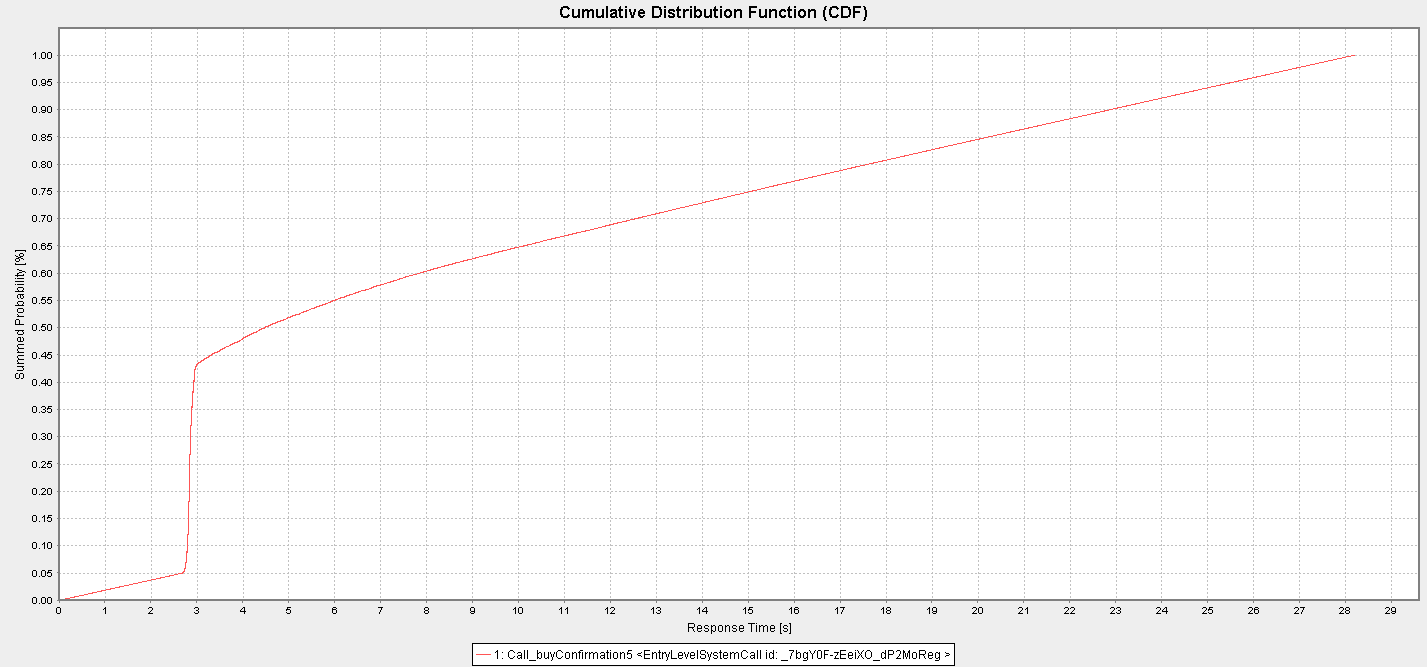
\includegraphics[width=17cm]{cloudstore-plain-cdf-1}
  \caption{\small{Función de distribución acumulativa de los tiempos de respuesta de la lógica de pagos en la versión original \emph{CloudStore}}}
  \label{fig:cloudstore-pcm-1}
\end{figure*}

Para obtener datos sobre el comportamiento de \emph{CloudStore} en AWS, se creó una prueba utilizando JMeter\footnote{\url{https://jmeter.apache.org}} en donde se realizaron 200 solicitudes durante un minuto al recurso Web \texttt{/payment} en la aplicación original (\emph{cloudstore-plain}), el cual es el que ejercita directamente la lógica de pagos y la comunicación con el \emph{gateway} de pagos. De acuerdo con los resultados obtenidos por la prueba de carga, el tiempo promedio de respuesta fue de 27 segundos. En la figura  \ref{fig:cloudstore-jmeter-plain-1} se muestra en detalle los tiempos de respuesta obtenidos durante la ejecución de la prueba.

\begin{figure}[h]
  \centering
  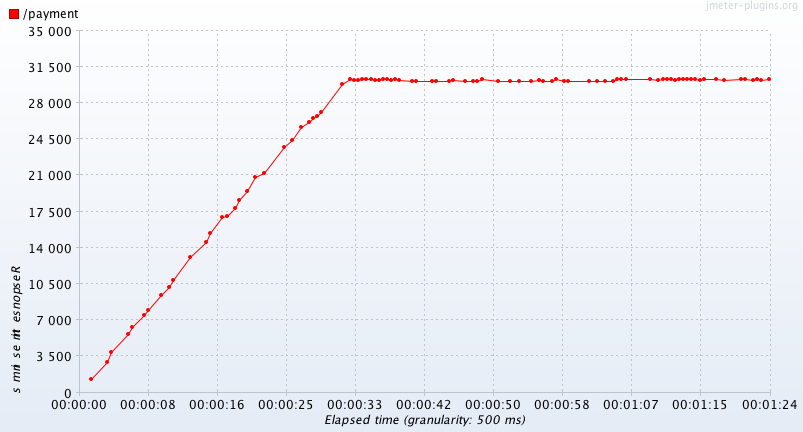
\includegraphics[width=9cm]{cloudstore-plain-aws-1}
  \caption{\small{Tiempos de respuesta del recurso web \texttt{/payment} en \emph{cloudstore-plain}}}
  \label{fig:cloudstore-jmeter-plain-1}
\end{figure}

De acuerdo a lo obtenido durante la simulación y a la prueba de carga, el modelo PCM de \emph{CloudStore} puede predecir el tiempo de respuesta de la lógica de pagos en un 95\%. Esto sugiere que el modelo PCM proporcionado de \emph{CloudStore} puede explicar el comportamiento de la aplicación.

\subsection{Pruebas sobre modelo PCM y aplicación adaptada para MOM en CloudStore}
Tomando como base el modelo PCM modificado de \emph{CloudStore} de la sección \ref{sec:cloudstore-mom} y utilizando las mismas pruebas que trae consigo la distribución de \emph{CloudStore}, se procedió a ejecutar las simulaciones con el fin de explorar la influencia de los nuevos componentes de MOM en el modelo. En la figura \ref{fig:cloudstore-pcm-jms-1} se muestra la función de distribución acumulada para los tiempos de respuesta esperados para las invocaciones de pagos.

\begin{figure*}[h]
  \centering
  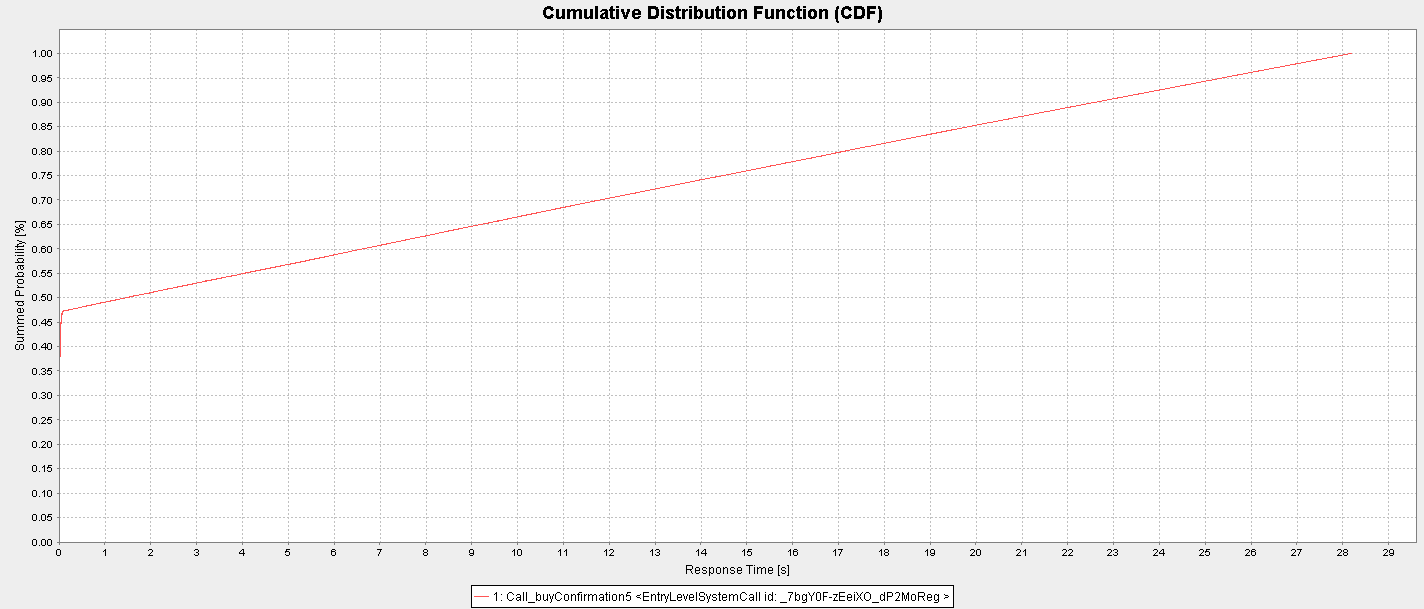
\includegraphics[width=17cm]{cloudstore-palladio-jms-cdf-1.png}
  \caption{\small{Función de distribución acumulativa de los tiempos de respuesta de la lógica de pagos en la versión adaptada con MOM de \emph{CloudStore}}}
  \label{fig:cloudstore-pcm-jms-1}
\end{figure*}

La misma prueba en JMeter que se realizó en la sección \ref{sec:pruebas-1} se utilizó para obtener los tiempos de respuesta a las invocaciones al recurso Web \texttt{/payment} sobre la aplicación adaptada con MOM/ActiveMQ (\emph{cloudstore-jms}). La figura \ref{fig:cloudstore-jmeter-jms-1} muestra los tiempos de respuesta obtenidos. De acuerdo con los resultados obtenidos por la prueba de carga, el tiempo promedio de respuesta fue de 43 segundos.

\begin{figure}[h]
  \centering
  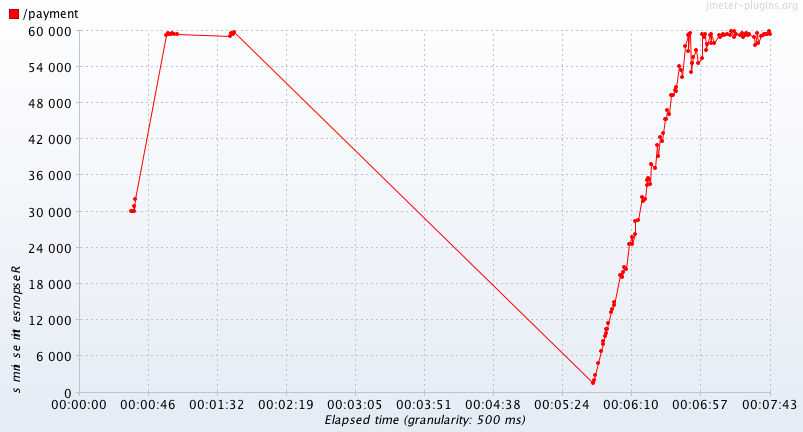
\includegraphics[width=9cm]{cloudstore-jms-aws-1}
  \caption{\small{Tiempos de respuesta del recurso web \texttt{/payment} en \emph{cloudstore-jms}}}
  \label{fig:cloudstore-jmeter-jms-1}
\end{figure}

Los resultados de las simulaciones en el modelo no logran explicar el comportamiento de la aplicación. Mientras que en las pruebas de carga el tiempo promedio de una invocación al recurso Web \texttt{/payment} tomó alrededor de 43 segundos, las simulaciones señalan que el 100\% de las invocaciones no deberían de tomar más de 29 segundos. Se modificaron otros parámetros en el modelo con el fin de explorar otros resultados pero al ejecutar las simulaciones se obtuvo resultados similares al mostrado en la figura \ref{fig:cloudstore-pcm-jms-1}. 

Como observación adicional, se pudo constatar que a pesar que el tiempo promedio obtenido en las invocaciones al recurso Web \texttt{/payment} fue mucho mayor en la aplicación adaptada con MOM que la aplicación original, el 100\% de las invocaciones fueron resueltas exitosamente (\texttt{200 - OK}), mientras que en la aplicación original se obtuvo varias respuestas de tipo \texttt{503 - Service Unavailable} cuando se efectuaba la comunicación con el \emph{gateway} de pagos. El \emph{gateway} de pagos en una aplicación Web secuencial escrita en Python y experimentó fallos al estar expuesta a llamados de forma concurrente. En la versión adaptada con MOM/ActiveMQ, las colas de mensajería ayudaron a poner un orden en las invocaciones al \emph{gateway} de pagos y esto hizo que el mismo pudiera procesar las invocaciones sin llegar a reportar errores.

\section{Conclusión} \label{sec:conclusion}
Este artículo presenta un enfoque exploratorio para modelar y simular \emph{middleware} orientado a mensajes basado en componentes y la influencia de estos en el rendimiento de una aplicación. Hace uso del \emph{Palladio Component Model}, un enfoque de modelado y simulación de arquitecturas de sofware basado en componentes.

Aunque el rendimiento de MOM ha sido estudiado y varios modelos se han propuesto, esto se ha tratado de manera aislada y no dentro del contexto de todo un sistema de software. Con el fin de evaluar esta influencia dentro de un sistema, se adaptó una aplicación para que use MOM y de esta forma poder observar cambios en el tiempo de respuesta durante su ejecución. La aplicación modificada es \emph{CloudStore}, una aplicación Web que emula una tienda de libros en línea y que fue desarrollada como parte del proyecto \emph{CloudScale}. Una de las ventaja de las aplicaciones que utlizan \emph{CloudScale} es que deben de tener un modelos de componentes basados en PCM para su procesamiento, la cual la convierte en una buena candidata ya que se puede partir de un modelo PCM base estable y probado.

Dos versiones de \emph{CloudStore} fueron publicadas en AWS: una con el código original y otra modificada para realizar comunicación basada en mensajes con un \emph{gateway} de pagos. El modelo PCM original de \emph{CloudStore} fue modificado con el fin de agregarle componentes para describir comunicación basada en mensajes de acuerdo a los modelos propuestos en \cite{happe-et-al}. Se ejecutaron simulaciones sobre los modelos PCM y pruebas de carga en las dos versiones de \emph{CloudStore}. Las resultados de las simulaciones en modelo original de \emph{CloudStore} pudieron predecir en un 95\% el comportamiento de las invocaciones al \emph{gateway} de pagos en la aplicación original, mientras que los resultados de las simulaciones en el modelo adaptado con componentes para MOM no logró predecir el comportamiento de la aplicación que realizada comunicación con el \emph{gateway} de pagos por medio medio de MOM. 
 
A pesar que los cambios introducidos en los modelos de \emph{CloudStore} no lograron explicar el comportamiento de la aplicación en producción, se considera que mayor trabajo futuro utilizando este enfoque de modelado y simulación puede llegar a dar con estimaciones más precisas del comportamiento de una aplicación utilizando MOM. PCM se considera un proyecto maduro y ha sido utilizado con éxito en otros sistemas, por lo que futuras experiencias y refinamientos en los modelos aquí expuestos pueden ser sujeto de mejoramiento para futuras investigaciones.


\begin{thebibliography}{00}
% 1
\bibitem{happe-et-al} Jens Happe, Holger Friedrich, Steffen Becker, and Ralf H. Reussner. \emph{A pattern-based performance completion for Message-oriented Middleware}. In Proceedings of the 7th international workshop on Software and performance (WOSP '08). ACM, New York, NY, USA, 165-176. 2008. DOI: \url{http://ezproxy.itcr.ac.cr:2075/10.1145/1383559.1383581} 

%2
\bibitem{woodside-et-al-2} Murray Woodside, Dorin Petriu, and Khalid Siddiqui. \emph{Performance-related Completions for Software Specifications}. In Proceedings of the 24th International Conference on Software Engineering, pages 22–32, New York, NY, USA, 2002.

%%3
%\bibitem{cloudscale-2} Sebastian Lehrig and Richard Sanders and Gunnar Brataas and Mariano Cecowski and Simon Ivanšek and Jure Polutnik. \emph{CloudStore — towards scalability, elasticity, and efficiency benchmarking and analysis in Cloud computing}. Future Generation Computer Systems, Vol 38, pages 115 - 126. 2018. DOI: \url{https://doi.org/10.1016/j.future.2017.04.018} 

%3
\bibitem{liu-gordon} Yan Liu and Ian Gorton. \emph{Performance prediction of J2EE applications using messaging protocols}. In Proceedings of the 8th international conference on Component-Based Software Engineering (CBSE'05), George T. Heineman, Ivica Crnkovic, Heinz W. Schmidt, Judith A. Stafford, and Clemens Szyperski (Eds.). Springer-Verlag, Berlin, Heidelberg, 1-16. 2005. DOI \url{http://ezproxy.itcr.ac.cr:2075/10.1007/11424529_1}

%4
\bibitem{chew} Chew, Zen Bob. \emph{Modelling Message-oriented-middleware Brokers Using Autoregressive Models for Bottleneck Prediction}. PhD Thesis. Queen Mary, University of London. 2013. \url{https://qmro.qmul.ac.uk/jspui/handle/123456789/8832}

%5
\bibitem{martinec-et-al} Tomáş Martinec, Lukáş Marek, Antonín Steinhauser, Petr Tůma, Qais Noorshams, Andreas Rentschler, and Ralf Reussner. \emph{Constructing performance model of JMS middleware platform}. In Proceedings of the 5th ACM/SPEC international conference on Performance engineering (ICPE '14). ACM, New York, NY, USA, 123-134. 2014. DOI: \url{https://ezproxy.itcr.ac.cr:2878/10.1145/2568088.2568096}

%6
\bibitem{alwakeel} S.S. Alwakeel and H.M. Almansour. \emph{Modeling and Performance Evaluation of Message-oriented Middleware with Priority Queuing}. Information Technology Journal, 10: 61-70. 2011. DOI \url{http://dx.doi.org/10.3923/itj.2011.61.70}

%7
\bibitem{woodside-et-al} Murray Woodside, Greg Franks, and Dorina C. Petriu. \emph{The Future of Software Performance Engineering}. Future of Software Engineering (FOSE '07), pages 171-187, May 2007. DOI 10.1109/FOSE.2007.32
 
%8    
\bibitem{performance-model-survey} Heiko Koziolek. 2010. \emph{Performance evaluation of component-based software systems: A survey. Perform}. Eval. 67, 8 (August 2010), 634-658. DOI: \url{http://ezproxy.itcr.ac.cr:2075/10.1016/j.peva.2009.07.007}     

%9
\bibitem{thijmen-thesis} Thijmen de Gooijer. \emph{Performance Modeling of ASP.Net Web
Service Applications: an Industrial Case Study}. Master's thesis, Malardalen University, Vasteras, Sweden, 2011.

%10
\bibitem{jit-et-al} Yan Jin, Antony Tang, Jun Han, and Yan Liu. \emph{Performance Evaluation and Prediction for Legacy Information Systems}. 29th International Conference on Software Engineering (ICSE'07), pages 540-549, May 2007.

%11
\bibitem{noorshams} Qais Noorshams. \emph{Modeling and Prediction of I/O Performance in Virtualized Environments}. PhD thesis, Karlsruhe Institute of Technology (KIT), 2015. URL: \url{http://digbib.ubka.uni-karlsruhe.de/volltexte/1000046750}

%12
\bibitem{jms20} Mark Richards, Richard Monson-Haefel, David Chappell. \emph{Java Message Service}. O'Reilly Media. Segunda Edición. 2009.

%13
\bibitem{cloudscale-2} Sebastian Lehrig and Richard Sanders and Gunnar Brataas and Mariano Cecowski and Simon Ivanšek and Jure Polutnik. \emph{CloudStore — towards scalability, elasticity, and efficiency benchmarking and analysis in Cloud computing}. Future Generation Computer Systems, Vol 38, pages 115 - 126. 2018. DOI: \url{https://doi.org/10.1016/j.future.2017.04.018} 

%14
\bibitem{cloudscale} Gunnar Brataas, Erlend Stav, Sebastian Lehrig, Steffen Becker, Goran Kopčak, and Darko Huljenic. 2013. \emph{CloudScale: scalability management for cloud systems}. In Proceedings of the 4th ACM/SPEC International Conference on Performance Engineering (ICPE '13), Seetharami Seelam (Ed.). ACM, New York, NY, USA, 335-338. 2013. DOI: \url{https://ezproxy.itcr.ac.cr:2878/10.1145/2479871.2479920}

\end{thebibliography}


%\subsection{Maintaining the Integrity of the Specifications}
%
%The IEEEtran class file is used to format your paper and style the text. All margins, 
%column widths, line spaces, and text fonts are prescribed; please do not 
%alter them. You may note peculiarities. For example, the head margin
%measures proportionately more than is customary. This measurement 
%and others are deliberate, using specifications that anticipate your paper 
%as one part of the entire proceedings, and not as an independent document. 
%Please do not revise any of the current designations.
%
%\section{Prepare Your Paper Before Styling}
%Before you begin to format your paper, first write and save the content as a 
%separate text file. Complete all content and organizational editing before 
%formatting. Please note sections \ref{AA}--\ref{SCM} below for more information on 
%proofreading, spelling and grammar.
%
%Keep your text and graphic files separate until after the text has been 
%formatted and styled. Do not number text heads---{\LaTeX} will do that 
%for you.
%
%\subsection{Abbreviations and Acronyms}\label{AA}
%Define abbreviations and acronyms the first time they are used in the text, 
%even after they have been defined in the abstract. Abbreviations such as 
%IEEE, SI, MKS, CGS, ac, dc, and rms do not have to be defined. Do not use 
%abbreviations in the title or heads unless they are unavoidable.
%
%\subsection{Units}
%\begin{itemize}
%\item Use either SI (MKS) or CGS as primary units. (SI units are encouraged.) English units may be used as secondary units (in parentheses). An exception would be the use of English units as identifiers in trade, such as ``3.5-inch disk drive''.
%\item Avoid combining SI and CGS units, such as current in amperes and magnetic field in oersteds. This often leads to confusion because equations do not balance dimensionally. If you must use mixed units, clearly state the units for each quantity that you use in an equation.
%\item Do not mix complete spellings and abbreviations of units: ``Wb/m\textsuperscript{2}'' or ``webers per square meter'', not ``webers/m\textsuperscript{2}''. Spell out units when they appear in text: ``. . . a few henries'', not ``. . . a few H''.
%\item Use a zero before decimal points: ``0.25'', not ``.25''. Use ``cm\textsuperscript{3}'', not ``cc''.)
%\end{itemize}
%
%\subsection{Equations}
%Number equations consecutively. To make your 
%equations more compact, you may use the solidus (~/~), the exp function, or 
%appropriate exponents. Italicize Roman symbols for quantities and variables, 
%but not Greek symbols. Use a long dash rather than a hyphen for a minus 
%sign. Punctuate equations with commas or periods when they are part of a 
%sentence, as in:
%\begin{equation}
%a+b=\gamma\label{eq}
%\end{equation}
%
%Be sure that the 
%symbols in your equation have been defined before or immediately following 
%the equation. Use ``\eqref{eq}'', not ``Eq.~\eqref{eq}'' or ``equation \eqref{eq}'', except at 
%the beginning of a sentence: ``Equation \eqref{eq} is . . .''
%
%\subsection{\LaTeX-Specific Advice}
%
%Please use ``soft'' (e.g., \verb|\eqref{Eq}|) cross references instead
%of ``hard'' references (e.g., \verb|(1)|). That will make it possible
%to combine sections, add equations, or change the order of figures or
%citations without having to go through the file line by line.
%
%Please don't use the \verb|{eqnarray}| equation environment. Use
%\verb|{align}| or \verb|{IEEEeqnarray}| instead. The \verb|{eqnarray}|
%environment leaves unsightly spaces around relation symbols.
%
%Please note that the \verb|{subequations}| environment in {\LaTeX}
%will increment the main equation counter even when there are no
%equation numbers displayed. If you forget that, you might write an
%article in which the equation numbers skip from (17) to (20), causing
%the copy editors to wonder if you've discovered a new method of
%counting.
%
%{\BibTeX} does not work by magic. It doesn't get the bibliographic
%data from thin air but from .bib files. If you use {\BibTeX} to produce a
%bibliography you must send the .bib files. 
%
%{\LaTeX} can't read your mind. If you assign the same label to a
%subsubsection and a table, you might find that Table I has been cross
%referenced as Table IV-B3. 
%
%{\LaTeX} does not have precognitive abilities. If you put a
%\verb|\label| command before the command that updates the counter it's
%supposed to be using, the label will pick up the last counter to be
%cross referenced instead. In particular, a \verb|\label| command
%should not go before the caption of a figure or a table.
%
%Do not use \verb|\nonumber| inside the \verb|{array}| environment. It
%will not stop equation numbers inside \verb|{array}| (there won't be
%any anyway) and it might stop a wanted equation number in the
%surrounding equation.
%
%\subsection{Some Common Mistakes}\label{SCM}
%\begin{itemize}
%\item The word ``data'' is plural, not singular.
%\item The subscript for the permeability of vacuum $\mu_{0}$, and other common scientific constants, is zero with subscript formatting, not a lowercase letter ``o''.
%\item In American English, commas, semicolons, periods, question and exclamation marks are located within quotation marks only when a complete thought or name is cited, such as a title or full quotation. When quotation marks are used, instead of a bold or italic typeface, to highlight a word or phrase, punctuation should appear outside of the quotation marks. A parenthetical phrase or statement at the end of a sentence is punctuated outside of the closing parenthesis (like this). (A parenthetical sentence is punctuated within the parentheses.)
%\item A graph within a graph is an ``inset'', not an ``insert''. The word alternatively is preferred to the word ``alternately'' (unless you really mean something that alternates).
%\item Do not use the word ``essentially'' to mean ``approximately'' or ``effectively''.
%\item In your paper title, if the words ``that uses'' can accurately replace the word ``using'', capitalize the ``u''; if not, keep using lower-cased.
%\item Be aware of the different meanings of the homophones ``affect'' and ``effect'', ``complement'' and ``compliment'', ``discreet'' and ``discrete'', ``principal'' and ``principle''.
%\item Do not confuse ``imply'' and ``infer''.
%\item The prefix ``non'' is not a word; it should be joined to the word it modifies, usually without a hyphen.
%\item There is no period after the ``et'' in the Latin abbreviation ``et al.''.
%\item The abbreviation ``i.e.'' means ``that is'', and the abbreviation ``e.g.'' means ``for example''.
%\end{itemize}
%An excellent style manual for science writers is \cite{b7}.
%
%\subsection{Authors and Affiliations}
%\textbf{The class file is designed for, but not limited to, six authors.} A 
%minimum of one author is required for all conference articles. Author names 
%should be listed starting from left to right and then moving down to the 
%next line. This is the author sequence that will be used in future citations 
%and by indexing services. Names should not be listed in columns nor group by 
%affiliation. Please keep your affiliations as succinct as possible (for 
%example, do not differentiate among departments of the same organization).
%
%\subsection{Identify the Headings}
%Headings, or heads, are organizational devices that guide the reader through 
%your paper. There are two types: component heads and text heads.
%
%Component heads identify the different components of your paper and are not 
%topically subordinate to each other. Examples include Acknowledgments and 
%References and, for these, the correct style to use is ``Heading 5''. Use 
%``figure caption'' for your Figure captions, and ``table head'' for your 
%table title. Run-in heads, such as ``Abstract'', will require you to apply a 
%style (in this case, italic) in addition to the style provided by the drop 
%down menu to differentiate the head from the text.
%
%Text heads organize the topics on a relational, hierarchical basis. For 
%example, the paper title is the primary text head because all subsequent 
%material relates and elaborates on this one topic. If there are two or more 
%sub-topics, the next level head (uppercase Roman numerals) should be used 
%and, conversely, if there are not at least two sub-topics, then no subheads 
%should be introduced.
%
%\subsection{Figures and Tables}
%\paragraph{Positioning Figures and Tables} Place figures and tables at the top and 
%bottom of columns. Avoid placing them in the middle of columns. Large 
%figures and tables may span across both columns. Figure captions should be 
%below the figures; table heads should appear above the tables. Insert 
%figures and tables after they are cited in the text. Use the abbreviation 
%``Fig.~\ref{fig}'', even at the beginning of a sentence.
%
%\begin{table}[htbp]
%\caption{Table Type Styles}
%\begin{center}
%\begin{tabular}{|c|c|c|c|}
%\hline
%\textbf{Table}&\multicolumn{3}{|c|}{\textbf{Table Column Head}} \\
%\cline{2-4} 
%\textbf{Head} & \textbf{\textit{Table column subhead}}& \textbf{\textit{Subhead}}& \textbf{\textit{Subhead}} \\
%\hline
%copy& More table copy$^{\mathrm{a}}$& &  \\
%\hline
%\multicolumn{4}{l}{$^{\mathrm{a}}$Sample of a Table footnote.}
%\end{tabular}
%\label{tab1}
%\end{center}
%\end{table}

%\begin{figure}[htbp]
%\centerline{\includegraphics{fig1.png}}
%\caption{Example of a figure caption.}
%\label{fig}
%\end{figure}

%Figure Labels: Use 8 point Times New Roman for Figure labels. Use words 
%rather than symbols or abbreviations when writing Figure axis labels to 
%avoid confusing the reader. As an example, write the quantity 
%``Magnetization'', or ``Magnetization, M'', not just ``M''. If including 
%units in the label, present them within parentheses. Do not label axes only 
%with units. In the example, write ``Magnetization (A/m)'' or ``Magnetization 
%\{A[m(1)]\}'', not just ``A/m''. Do not label axes with a ratio of 
%quantities and units. For example, write ``Temperature (K)'', not 
%``Temperature/K''.

%\section*{Acknowledgment}
%
%The preferred spelling of the word ``acknowledgment'' in America is without 
%an ``e'' after the ``g''. Avoid the stilted expression ``one of us (R. B. 
%G.) thanks $\ldots$''. Instead, try ``R. B. G. thanks$\ldots$''. Put sponsor 
%acknowledgments in the unnumbered footnote on the first page.

%\section*{References}
%
%Please number citations consecutively within brackets \cite{b1}. The 
%sentence punctuation follows the bracket \cite{b2}. Refer simply to the reference 
%number, as in \cite{b3}---do not use ``Ref. \cite{b3}'' or ``reference \cite{b3}'' except at 
%the beginning of a sentence: ``Reference \cite{b3} was the first $\ldots$''
%
%Number footnotes separately in superscripts. Place the actual footnote at 
%the bottom of the column in which it was cited. Do not put footnotes in the 
%abstract or reference list. Use letters for table footnotes.
%
%Unless there are six authors or more give all authors' names; do not use 
%``et al.''. Papers that have not been published, even if they have been 
%submitted for publication, should be cited as ``unpublished'' \cite{b4}. Papers 
%that have been accepted for publication should be cited as ``in press'' \cite{b5}. 
%Capitalize only the first word in a paper title, except for proper nouns and 
%element symbols.
%
%For papers published in translation journals, please give the English 
%citation first, followed by the original foreign-language citation \cite{b6}.



\end{document}
xccz=